\chapter{绪\hskip 0.4cm 论}
\label{ch1}

\section{研究背景及意义}
信息物理融合系统(Cyber Physical System,CPS)\cite{wangzhongjie2011cpssurvey}是一种复杂的异构系统,主要具有以下两个特征:1)不确定性:该系统面向开放环境,受多种不确定因素影响,如天气突变、信号误差、人为失误等,因此在设计该系统时,我们要充分考虑多种不确定性的因素,以保障CPS 在不确定环境下的可信性;2)异构性:该系统除了包含计算机系统之外,还结合了机械、环境、土木、电子、生物、化学、航空等诸多工程领域的模型和方法,且各领域深度的融合,因此我们不仅仅需要设计和建模各个工程领域的模型,更要充分考虑各个领域之间的交互问题。因此,由于CPS的不确定性和异构性,使CPS的建模分析及验证面临巨大的挑战,已有的CPS研究已经针对CPS的建模、仿真做了大量的工作并相应的有了一些工具的支持,例如基于时间自动机理论的UPPAAL\cite{bulychev2012uppaal}可以很好的建模和验证系统的基于时间的行为,基于马尔科夫模型的Prism\cite{kwiatkowska2011prism}对概率系统的建模和验证提供了很好的支持,Modelica \cite{Fritzson1998Modelica}、Simulink\cite{zuliani2013bayesian} 等工具支持对连续的物理系统提供较好的建模仿真等等。然而,以上工作在解决CPS的建模仿真及验证问题上各有优势及不足。因此,想要更好的支持CPS系统各种性质的建模、仿真和验证,我们需要整合多种特定领域模型工具的建模、仿真及验证优势。为了解决这一问题,GEORG, H等人在论文\cite{Georg2014Analyzing}中提出了两种方法:一种是设计统一的建模仿真平台,该平台可以结合所有领域模型的优势并支持所有领域模型的建模仿真;另一种是使用协同仿真技术,仍然是在各个领域模型的建模工具中进行建模,然后将各个领域建模工具建模出的模型根据统一标准转化为一种标准模型,最后根据这一标准提供的接口在仿真过程对模型进行仿真。Georg, H等人在文中也提到,第一种方案实现起来比较困难,所以建议使用第二种方案。经过协同仿真过程之后,我们可以得到不同领域模型融合在一起仿真的迹(trace),由于仿真迹的可读性不高,通过对仿真迹进行直接观察我们很难评估分析系统的行为。因此,LEGAY A等人提出了统计模型检测方法(Statistical Model Checking,SMC)\cite{Legay2010Statistical},该方法以模型的仿真迹和验证属性(Property)作为输入,最终将得到模型满足这一属性的概率值。统计模型检测方法提出以来,主要是用来对特定领域模型的行为进行定量的评估分析,在本文中我们用该方法来评估分析多个模型协同之后的行为。

本文提出了一种基于协同仿真及统计模型检测的信息物理融合系统定量评估分析方法,在该方法中我们使用协同仿真技术来对多个领域模型进行融合仿真并得到仿真的迹,然后对整个系统设计需要验证的属性,最后将仿真迹和验证属性输入到统计模型检测器中进行评估分析。对于该方法,我们主要需要解决两个问题,也是本文的两个重要的贡献点:(1)需要保证多个领域模型进行协同仿真时的正确性,即需要对多个模型进行协同时的协同行为进行验证;(2)由于统计模型检测需要消耗大量的仿真迹,且在协同仿真时产生仿真迹的过程尤为耗时,使得整个验证时间需要极大的时间开销,因此我们需要对统计模型检测算法进行改进,以更快的完成验证过程。解决了以上两个问题之后,我们本文提出的方法就可以很好的结合多种建模仿真的优势,并为准确高效的对CPS系统的建模、仿真和定量评估分析提供有效的支持。 


\section{国内外研究现状}

\subsection{信息物理融合系统}
信息物理融合系统的概念最早是由美国自然基金委提出,之后便获得了国内外的广泛关注。各个国家的科研人员从CPS的建模、验证分析等不同方面展开了深入的研究。CPS从2005年提出至今,它的发展得到了多国政府的大力资助和支持,并成为学术界、科技界研究的重点方向,具有很高的科学研究意义。同时,CPS也在工业界有了大量的案例应用,具有广阔的应用前景和商业价值。在美国,近些年举办了多次CPS的科研会议和研讨活动,针对CPS的理论、性能及安全性等问题展开了深入的探讨。美国科研人员的研究热点主要涉及嵌入式系统、网络信息安全等方面,并已经取得了较好的研究成果。例如:哥伦比亚大学伯克利分校设计的PTOLEMY平台对CPS系统的架构建模和仿真提供了工具支持。麻省理工学院 (Massachusetts Institute of Technology, MIT)设计了分布式智能机器人花园,提高了CPS各个节点之间的交互和实时通讯的效率。宾夕法尼亚工程学院了汽车导航软件GrooveNet,为车辆CPS系统的建模和仿真提供了一个良好的建模和仿真平台。Carnegie Mellon 大学将支持向量机预测模型和马尔科夫状态控制等方法应用于智能电网CPS系统的建模之中,来实现智能电网的调度控制。在欧洲,对于CPS的研究主要集中在理论研究方面。例如:在2008年,欧盟启动了 ARTEMIS (Advanced research and technology for embedded intelligence and systems) 项目, 将CPS作为一个重点的研究方向, 并创办了 “International Journal of Cyber-Physical Systems”专刊。法国自动化研究所设计的GEMOC平台对信息物理融合系统的建模提供了有效的支持。在中国,于2008年在北京召开了IEEE嵌入式研讨会, 将CPS作为接下来的重点研究方向。2010年, 国家863计划信息技术领域办公室和专家组在上海举办了 “CPS发展战略论坛”, 对CPS给以高度关注。武汉大学信息资源研究中心提出了结合云计算和下一代互联网的理念, 进行 CPS 语义中间件的设计, 研了究CPS 网络互联和自主交互等技术。华东师范大学使用形式化的方法对CPS进行了建模,并对其可信性进行了验证分析。此外, 清华大学、天津大学、同济大学等多所研究机构也对CPS进行了深入研究。


\subsection{分布式技术}
分布式计算技术是计算机发展过程中产生的一项科学技术,主要工作原理是通过多台计算机的分布式连接实现数据的综合处理,旨在通过多台计算机的强大的工作能力来分解复杂问题,解决一些计算难题。分布式计算技术的具体特征表现如下:首先,分布式计算能够合理分配计算内容,实现多台计算机共同工作,节约设备成本,提高工作效率。其中最核心的内容在于能够为计算程序寻找最合适的计算机来完成工作。目前,计算机领域内关于分布式计算的技术已有数百种之多,但多数并没有密切的联系,这种缺乏系统管理和统一行业规定的技术并不利于日后的广泛发展。另外,分布式计算技术主要是通过科学算法的研究,形成一种独特的计算模型,确保其超长的数据处理能力,这种发展规律导致大多数用户只单纯研究如何集结更多闲置计算机来完成实际数据的处理,并没有考虑如当某些计算机丧失处理能力后的数据归属问题。那么,就要求研究者对分布式计算技术进行更加深入、系统的研究,目前,通过虚拟网络运营机制来实现大批量数据的共同处理以及如何实现用户间数据的高速共享以初具规模。如何更大规模的集结剩余计算力量、如何科学系统的管理共享数据资源、如何更大程度的节省计算资源成本成为当今社会研究分布式计算技术的重要课题。

\subsection{协同仿真}
由于CPS包含信息和物理两个部分,并涉及各个领域,因此,对于CPS的各个部分的建模在不同的领域都有相应的工具及方法支持。如果将CPS各个部分联系在一起进行仿真分析通常有两种方法: 1)开发一个统一的CPS建模平台,将CPS的所有相关部分都在此平台建模仿真分析2)将CPS的各个部分在不同的工具中建模,使用协同仿真技术[22,23]联合CPS的各个部分进行仿真。方法一到目前为止实现起来较为复杂,所以通常采用第二种方法较多,但协同仿真技术在实际的仿真中需要消耗较多的时间,针对这一问题,我们之前提出了[24]有效的提高了协同仿真的效率。

\subsection{统计模型检测}
人们利用统计知识来分析系统由来已久,SMC技术即建立在蒙特卡洛模拟、假设检验等统计方法之上,通过统计分析系统仿真运行的Trace来验证系统属性满足的情况。它最早被Sen等人提出用来验证黑盒系统\cite{sen2004statistical},即Single Sampling Plan(SSP)算法的雏形,其难点在于确定算法收敛所需的Trace总样本数量$N$以及接受原假设的阈值$C$;Younes等人在博士论文\cite{younes2005verification}中提出一种二叉搜索的算法来近似得到所需的$n$和$c$,并指出了\cite{sen2004statistical}中验证黑盒系统方法的一些错误。基于Wald的Sequential Probability Ratio Test(SPRT)\cite{wald1945sequential}原理,Younes等人还提出了基于对数的SPRT实现算法\cite{younes2005verification,younes2006statistical},用以验证系统;该方法可以最小化算法所需Trace的样本数量。SSP与SPRT用以解决定性验证问题,回答了“系统$S$满足属性$\phi '$的概率是否大于或等于某个概率阈值$\theta$”这个问题,即$S \models P_{\geq \theta} (\phi ')$。与定性算法不同,定量算法可以直接返回$S$满足$\phi '$的概率$p$,如Approximate Probabilistic Model Checking(APMC)\cite{herault2004approximate},通过计算$x/n$来计算$p$(其中$x$和$n$分别表示所需的Trace正样本数量和总数量),并通过Chernoff-Hoeffding界来限定结果的误差范围。随后,Zuliani、Clarke等人基于贝叶斯统计又提出了两个新SMC实现算法:Bayesian Hypothesis Testing(BHT)和Bayesian Interval Estimation(BIE)\cite{jha2009bayesian,zuliani2013bayesian},前者基于贝叶斯假设检验解决定性验证问题,后者基于贝叶斯区间估计解决定量评估问题。

从SSP、SPRT、APMC到BHT、BIE,SMC算法所需Trace数量逐渐减少,效率逐渐提高。为了进一步探索SMC技术,许多人将数值方法与统计方法相结合\cite{bogdoll2011partial,pavese2013automated},来进一步提升SMC效率或解决一些SMC难以应付的问题,如非确定性问题(Non-determinism)。研究SMC非确定性算法的还有Henriques等人,其博士论文讨论了如何用概率方式近似解决非确定性问题\cite{henriques2012statistical}。SMC善于验证有界(通常指时间约束,即time-bounded)的属性,因此传统模型检测中的无界“Until”属性的SMC验证方法也是研究热点之一,He、Jennings等人提出了一种将无界“Until”验证转化为有界“Until”的方法以解决此问题\cite{he2010bounded,jennings2012two}。由于SMC基于系统仿真结果,所以也不可避免地引入了仿真领域的问题,比如小概率事件在Trace中出现概率极低,使得验证过程需要产生Trace的数量过多而效率低下。Jegourel、Legay等人基于重要性取样(Importance Sampling)和重要性分割(Importance Splitting)技术提出了面向小概率属性验证的SMC算法\cite{jegourel2012cross,jegourel2013importance},大大减少了验证所需的Trace样本数量;解决类似问题还可以借助于机器学习技术,如\cite{du2015smc4rare}借助支持向量机预测事件,\cite{kumar2014efficient}借助贝叶斯推断预测事件,都可以提高SMC的效率。除此之外,SMC还有一些特殊的应用场景,如黑盒系统\cite{sen2004statistical}、异构系统\cite{basu2010statistical,vodenvcarevic2012learning},允许在系统内部结构和行为未知的条件下分析系统。

Ymer\cite{younes2005ymer}和Vesta\cite{sen2005vesta}是最早实现SMC的验证工具。Vesta采用了极易实现并行化的SSP算法的一个变种,Ymer采用的SPRT算法很快也被Younes证明同样能够被并行化。Ymer在实验中的效率高于Vesta;此外,Vesta还支持了无界“Until”的验证。目前最流行的支持SMC的验证工具则是UPPAAL-SMC\cite{bulychev2012uppaal}和Prism\cite{kwiatkowska2011prism},UPPAAL-SMC和Prism都实现了定性的SPRT算法,同时都实现了基于置信区间(Confidence Interval,CI)\cite{brown2001interval}的定量算法(文献\cite{pires2008interval}对不同版本的CI统计算法进行了对比,并根据需求的不同,给出了方法选择的建议)。UPPAAL-SMC的建模基于PTA或SHA,使用图形化建模,用户友好,对于时间和连续行为的支持较好;Prism则使用Reactive Modules Language(RML)建模,对随机(如马尔科夫链)和非确定性(如马尔科夫决策过程)模型的验证支持较好。Plasma Lab\cite{boyer2013plasma}是新出现的一款纯SMC工具,同样支持RML建模,并实现了多种SMC算法(包括重要性取样和分割等面向小概率事件的算法)。Plasma Lab允许用户以插件集成的方式为其添加新的模型输入和验证算法,如Simulink的集成。

\section{本文技术路线及主要研究内容}
信息物理融合系统是异构系统,本文针对这种异构系统的验证提出了一种解决方案,图\ref{pa-fra}为本文的技术路线图,本文的技术路线大致如下:

(1)我们通过对该系统进行分析,提取出该系统的信息部分(Cyber part)和物理部分(Physical part),除此之外我们根据自己需要验证的行为属性定义约束(Constraint)。

(2)使用SysML\cite{•} 建模语言对提取出的信息部分和物理部分进行建模,将信息系统和物理系统的组件使用SysML的BDD(SysML Block Definition Diagram )图进行建模,同时使用SysML的IBD(SysML Internal Block Diagram)图来描述系统中各个组件之间的关联。

(3)SysML只是用来建模组件内部结构和组件之间的关联,该模型不可直接进行仿真运行,因此我们将SysML BDD图建模的模型使用FMU进行实现,同时将SysML IBD图描述的系统组件关系转化为FMU之间相互依赖的接口配置文件,此时,我们只需要再设计好协同仿真的主算法(Master Algorithm)就可以进行异构系统的协同仿真。然而,在进行协同仿真之前,我们首先要保证各个FMU之间的协同是正确的,要确保FMU之间协同行为的正确性,我们需要验证主算法的正确性及各个FMU之间的连接顺序及数据交换的正确性。在本文中,我们基于时间自动机设计了一个协同行为正确性验证的验证器,我们将系统的多个FMU、协同仿真的主算法以及FMU之间的接口配置文件输入到该协同行为的验证器之中即可验证当前系统协同行为的正确性,如果验证通过则说明我们当前的模型即为正确的模型,如果验证不通过,则需要修改当前系统的协同行为,直到得到验证通过的模型之后再输入到仿真器中进行仿真。

(4)我们在进行系统的验证分析时,首先需要验证的系统模型,同时我们还需要验证的属性(Property),我们将(1)中得到的约束进行形式化描述,即可得到验证属性(该验证属性根据约束的不同可以是BLTL/ALTL/GSCL等等)。

(5)将通过第三步验证的模型(Verified Model)及第四步得到的验证属性输入到异构系统验证器(co-verification)之中进行验证分析,首先将模型输入到仿真器(Simulator)之中进行仿真或协同仿真(Co-simulation)并得到仿真迹(Traces),然后将得到的仿真迹和验证属性输入到模型验证器(Checker)之中来验证该迹是否满足某条特定的验证属性,得到结果满足为1,不满足为0,我们将该验证是否满足的结果称为观察值(Observations),多条仿真迹对于一条特定的验证属性会得到多个观察值。最后将得到的观察值输入到统计分析算法中进行统计分析,并得到评估结果。
\begin{figure}[htbp]
	\centering
	{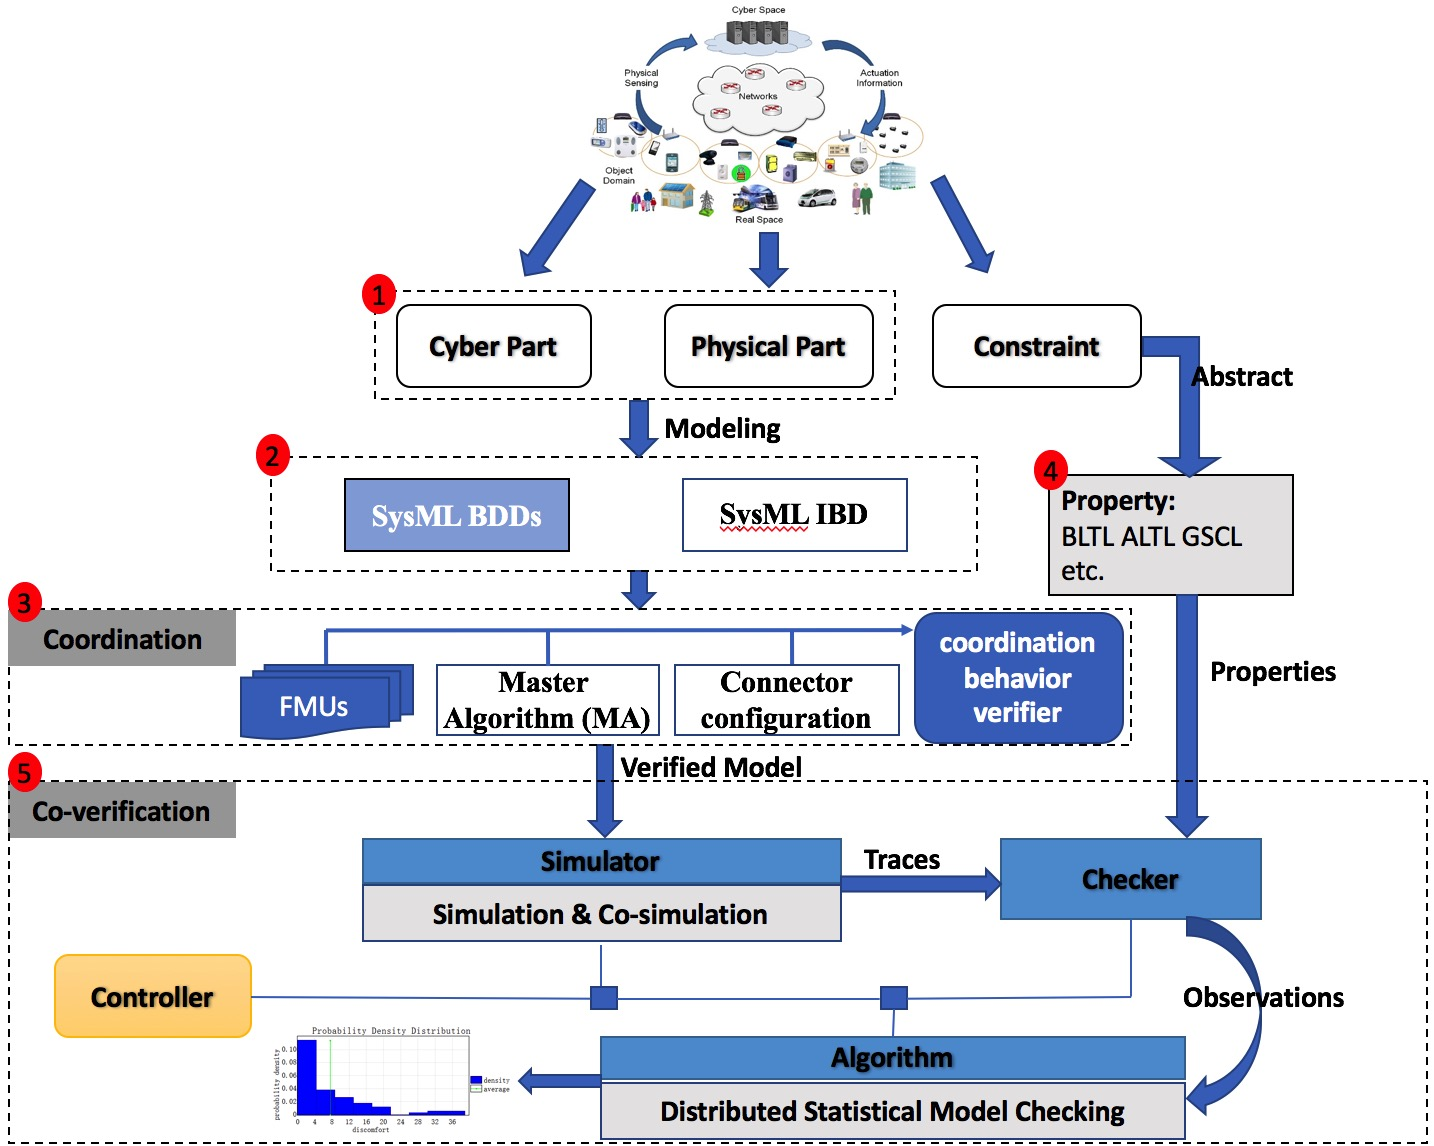
\includegraphics[width=5.0in]{fig/1/paper-framework.jpg}}
	%\vspace{0.10in}
	\caption{论文技术路线图}\label{pa-fra}
\end{figure}

\textbf{本文的具体研究内容和贡献点总结如下}:
\begin{enumerate}
	\item 使用SysML建模语言建模整个系统的架构,使用SysML的BDD图建模系统组件,使用SysML的IBD图来描述系统中各个组件的关联关系。
	\item 基于FMI标准实现SysML描述的系统模型,将SysML的BDD图建模的系统组件包装成FMU,并将各个组件的关联关系转化为FMU之间的接口配置文件。
    \item 使用时间自动机理论验证了基于FMI标准的多个组件的协同行为,使用时间自动机将协同仿真的主算法进行形式化描述,并使用UPPAAL \cite{•} 模型检测器来验证主算法的正确性;提出了一种从FMU到时间自动机的映射标准,通过此标准用时间自动机将多个FMU进行编码,并用时间自动机之间的通道(channel)来描述多个FMU之间的关联关系,最终将多个FMU及FMU之间的关联关系使用一个时间自动机网络进行了描述,将该时间自动机网络输入到UPPAAL之中进行验证从而来验证协同行为的正确性。
    \item 将验证属性用BLTL/ALTL/GSCL等形式化语言进行描述。
    \item 提出了一种基于抽象和学习的分布式统计模型检测算法,大大提高了统计模型检测的效率。
\end{enumerate}

\section{本文组织结构}
本文共分七章,组织结构如下:

第一章介绍了本文的研究背景及意义,并从四个方面阐述了该研究领域的国内外研究现状,其中包括信息物理融合系统的形式化建模、分布式技术、协同仿真及统计模型检测的研究现状。之后,给出了本文的技术路线和主要贡献点。最后,总结了论文组织结构。

第二章介绍了相关预备知识。首先给出了信息物理融合系统的主要概念,并详细讨论了我们本文关注的信息物理融合系统的异构性;之后,给出了概率有界线性时态逻辑和时间自动机的形式化描述,并给出了基于FMI标准的协同仿真通用接口。

第三章介绍了基于时间自动机理论来验证异构系统协同行为正确性的方法,首先我们给出了该方法的技术框架,之后我们详细描述了如何用时间自动机理论来验证协同仿真的主算法,以及如何验证整个异构系统的协同行为的正确性。

第四章重点阐述了如何用统计模型检测算法来对异构系统进行验证分析,也是本文的主要内容。首先,介绍了如何基于FMI标准对异构协同进行协同仿真并得到仿真迹,然后提出了一种基于抽象和学习的统计模型检测算法来提高统计模型检测的效率。最终,我们将协同仿真和该高效的统计模型检测算法进行结合,以此来对异构系统进行验证分析。

第五章主要介绍工具及程序实现。首先简单介绍了我们自己的CPS建模分析平台——Modana,之后给出了基于Modana平台的异构系统验证工具(Co-SMC工具)。最后,给出了Co-SMC工具的详细设计及程序实现。

第六章给出了两个案例,通过使用本文提出的方法对这两个案例进行建模、仿真和分析来验证本文提出方法的有效性。

第七章为总结和展望,总结了本文提出的基于分布式统计模型检测的异构系统验证方法,并讨论了其优点和不足,指出了未来要进一步进行研究的工作。
\section{本章小结}
本章首先说明了选题的背景和意义,指出了由于CPS的异构性而导致CPS系统的验证分析面临巨大挑战;接着介绍了信息物理融合系统的形式化建模、分布式技术、协同仿真及统计模型检测的研究现状;最后给出了本文的技术路线、主要贡献点和组织结构。下一章将介绍本文涉及到的预备知识及概念。
